% ___________________________________________________________________________
% |#########################################################################|
% |                                                                         |
% | The Manual for the C++ Reference Manual Style   cc_manual.tex           |
% | -------------------------------------------------------------           |
% |                                                                         |
% | 02.09.1996   Lutz Kettner   kettner@acm.org                             |
% | Zurich, Switzerland                                                     |
% | $Revision$                                                       |
% | $Date$                                            |
% |_________________________________________________________________________|
% |#########################################################################|

% The style is compatible with LaTeX2e:
\documentclass[12pt]{article}
\usepackage{latexsym}
\usepackage{amssymb}
\usepackage{path}
\usepackage{epsfig}
\usepackage{cc_manual}
\usepackage{latex_converter}
\usepackage{makeidx}
% \makeindex

%\pagestyle{empty}
\textwidth 15.4cm 
\textheight 24 cm
\topmargin -14mm       
\evensidemargin 3mm 
\oddsidemargin 3mm


\parindent0em
\setlength{\parskip}{1.4ex}

\sloppy

{
  \begingroup
    \catcode`\|=0
    \catcode`\[=1
    \catcode`\]=2
    \catcode`\{=12
    \catcode`\}=12    
    \catcode`\\=12    
    |gdef|Open[[|tt {]]
    |gdef|Close[[|tt }]]
    |gdef|Backslash[[|tt \]]
  |endgroup
}

\newcommand{\Mindex}[1]{\index{#1@\protect\Backslash{\tt #1}}}
\newcommand{\TTindex}[1]{\index{#1@{\tt #1}}}
\newcommand{\Dindex}[1]{#1\index{#1}}

\def\ind{\hspace*{7mm}}

% ----------------------------------------------------------------------
\title {{\tt cc\_extract} and {\tt cc\_check}\\[2mm]
        Extracting Sources from \CC\ Reference Manuals}

\author{Lutz Kettner}

\date{\ccRevision. \ccDate}

\begin{document}

\maketitle

\tableofcontents
\thispagestyle{empty}
\clearpage
\thispagestyle{empty}
~\vfill

% ___________________________________________________________________________
% |#########################################################################|
% |                                                                         |
% | The Manual for the C++ Reference Manual Style  disclaimer.tex           |
% | -------------------------------------------------------------           |
% |                                                                         |
% | 02.09.1996   Lutz Kettner   kettner@acm.org                             |
% | Zurich, Switzerland                                                     |
% | $Id$                                                       |
% | $Date$                                            |
% |_________________________________________________________________________|
% |#########################################################################|

% General disclaimer, copyright notice, and acknowledgements.

{\bf Note}

{\small These \LaTeX\ style and tools were created during the writing
  of the first versions of the CGAL Kernel Reference Manual and they
  are still evolving. New features are continuously added (even if
  this runs on low priority), so it might happen that the features
  implemented in the style file are non orthogonal, ugly named, and
  inconsistent. Please report errors, anomalies, and suggestions for
  improvements to {\tt <kettner@inf.ethz.ch>}. Please check the latest
  release, for example, available for members on the CGAL Home Page at
  {\tt <http://www.cs.uu.nl/CGAL/Members/>}.}\vspace{2ex}

{\bf Acknowledgements} 

{\small The CGAL Kernel is a group effort \cite{Fabri96,Fabri99} and
  so is the reference manual style, the \LaTeX\ to HTML converter and
  the related tools. I would like to thank Andreas Fabri, Geert-Jan
  Giezeman, Stefan Schirra, and Sven Sch\"onherr for all the
  suggestions and improvements, Susan Hert for taking over maintenance
  of this package, and the LEDA\TTindex{LEDA} group for their manual
  layout \cite{Naeher95} that we have mimicked here.}\vspace{2ex}

{\bf Copyright \copyright\ 1996,1997,1998,1999\\
Lutz Kettner}

{\small Permission to use, copy, and distribute this software and its
  documentation for non-comercial purpose is hereby granted without
  fee, provided that the above copyright notice appear in all copies
  and that both that copyright notice and this permission notice
  appear in supporting documentation.  I make no representations about
  the suitability of this software for any purpose.  It is provided
  "as is" without express or implied warranty.}



\cleardoublepage\setcounter{page}{1}

% ----------------------------------------------------------------------
\section{Introduction}

The tools for writing \CC\ reference manuals are arranged around a
\LaTeX\ style file called {\tt cc\_manual.sty}. The style provides
three groups of macros. The first group is a set of commonly used
abbreviations such as \verb+\R+ for \R. The second group helps to
structure the text with subtitles such as \verb+\ccDefinition+ or
\verb+\ccPrecond+.  The third group handles \CC\ declarations and
formats the declarations nicely. The \LaTeX\ to {\tt HTML}
converter~\cite{k-lhcll-99} fully supports the {\tt
  cc\_manual.sty}.\TTindex{cc\_manual.sty}\TTindex{HTML}

A set of \Dindex{tools} is dedicated to achieve \Dindex{consistency}
between the manual and the current implementation. A \Dindex{software
  engineering} process like the {\em \Dindex{waterfall model}\/} or
the {\em \Dindex{spiral model}\/} \cite{Fairley85} differentiates the
task of software development into design and implementation (among
other steps).  The result of the design phase is the specification,
here a \CC\ reference manual. The result of the implementation phase
is the source code and an additional implementation documentation (not
to be confused with the reference manual). \index{web tools} Web tools
\cite{Knuth84,Knuth94,Williams92} may be used to combine
implementation and its documentation.

The specification in the reference manual contains \CC\ declarations
that are repeated in the {\tt *.h} header files of the implementation.
The syntax in the {\tt *.tex} reference manual files uses \CC\ style
declarations to simplify the task of the manual authors (no additional
syntax) and the task for tools when processing the manual.  In
conformance with the development process the {\tt
  cc\_extract}\TTindex{cc\_extract} tool transforms the specification
to the declaration part of a {\tt *.h} header file. Neither a complete
{\tt *.h} header file is written in the manual nor a {\tt *.h} header
file is used for writing the manual.  A couple of declarations and
definitions have to be in an {\tt *.h} header file but must not be in
any specification (e.g. private class members or inline function
definitions). The second reason for this is more a matter of taste. It
is the idea of the web tools \cite{Knuth84} to write code within the
documentation instead of writing comments within code. Furthermore, if
the implementation is done with \Dindex{web tools}, the manual
specification would appear as a \CC\ comment within a {\tt *.h} header
file within a web file -- the second nesting level.

When the specification evolves as indicated by the \Dindex{software
  engineering} {\em cycle model}, the {\tt *.h} header files has to be
kept updated. An automatic {\em splicing mechanism\/} is possible, but
has not been developed so far. A {\em cut-and-paste\/} approach can be
used for the moment. Experience from practice indicates that the {\tt
  *.h} header files might get changed without updating the
specification in the manual (so not as clean as in the software
engineering {\em cycle model}).  Here, the {\tt
  cc\_check}\TTindex{cc\_check} tool can test whether all declarations
within a specification are currently contained within a {\tt *.h}
header file. Nonetheless, we believe in the benefits of keeping design
and implementation tasks separated and encourage this by keeping the
specification in its extra file and not mangled with the
implementation.\footnote{A side effect is that the file change date of
  the {\tt *.tex} file indicates changes in the specification, which
  is not true for the file change date of a {\tt *.h} header file.}

Both tools, {\tt cc\_extract} and {\tt cc\_check}, are documented in
this manual. The \LaTeX\ style file, {\tt cc\_manual.sty}, is
documented in~\cite{k-clswr-99}. The \LaTeX\ to HTML converter is
documented in~\cite{k-lhcll-99}.  An overview of the files involved
and the tools is given in Figure~\ref{ToolsOverviewFig}.

\def\figuretopindent{\vspace{2ex}}

\begin{figure}
    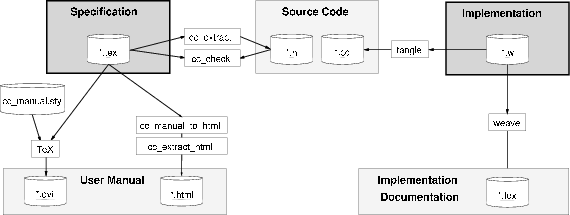
\psfig{file=tools_overview.ips,width=\textwidth}%
    \caption{The files and tools involved in the manual writing
      process.\index{files}\index{tools}}
    \label{ToolsOverviewFig}\figuretopindent
\end{figure}

The next section describes the {\tt cc\_extract} tool in detail.
Thereafter in Section~\ref{sectionChecker}, the {\tt cc\_check} tool
is explained.  The installation of these tools is not described in
this manual. Please refer to the {\tt README} and {\tt INSTALLATION}
files that are shipped with the distribution.

{\bf Note:} Both tools are in a less developed state than the \LaTeX\ 
style file or the \LaTeX\ to HTML converter.

% ----------------------------------------------------------------------
\section{Extracting Declarations from a Manual with {\tt cc\_extract}}
\label{sectionExtract}
\index{extract declarations}\index{declaration extraction}
\index{tools}
\TTindex{cc\_extract}

The {\tt cc\_extract} program reads a specification and writes all
declarations to the standard output. The output is in \CC\ format,
i.e., the declarations are copied literally and the documentation is
put in \CC\ comments. The documentation also is made a bit more
readable by translating several \LaTeX\ macros to ASCII text. The
synopsis for the program is:

\ind{\tt cc\_extract [<options>] [<infile> ...]}

Multiple input files are processed sequentially and the output is
concatenated. If no input file is given the program reads from the
standard input. Available options are:

\begin{tabular}{ll}
    {\tt -nomc}  & Suppress the output of main comments. \\
    {\tt -nosc}  & Suppress the output of subsidiary comments. \\
    {\tt -noc}   & Suppress the output of any comments (main and subsidiary).\\
    {\tt -trace} & Produce a debug trace from the {\tt bison} parser. \\
    {\tt -h, -help} & A short usage message and a summary of the options.
\end{tabular}

In principle, the main text of the specification is not converted to
\CC\ comments. Within class declarations, the main text is converted
to main comments that can be suppressed with {\tt -nomc}. The second
argument of declarations, which is formatted in the third column as
documentation, is converted to subsidiary comments that can be
suppressed with {\tt -nosc}. No comments at all are converted with the
option {\tt -noc}. The {\tt bison} parser trace is most likely
unreadable for users who are unexperienced with grammars. Nonetheless,
this trace can be very useful to figure out why a certain keyword is
not recognized in a certain context. The entries in the trace refers
to the {\tt extract\_syntax.output} file produced by {\tt bison}
parser generator. It is located in the source code directory of the
{\tt cc\_extract} program.

The {\tt cc\_extract\_include} program reads a specification and
writes all \verb+\ccInclude+ macros converted to C preprocessor
includes to the standard output. The synopsis for the program is:

\ind{\tt cc\_extract\_include [<infile> ...]}
\TTindex{cc\_extract\_include}\index{include file extraction}

A short example demonstrates the {\tt cc\_extract} program. A
specification file with a short class and two declarations is given.

{\footnotesize
\begin{verbatim}
    A short main text which is not converted.

    \begin{ccClassTemplate}{A<T>}
        A main text within a class declaration. References to the
        classname \ccClassName\ are possible. Math mode, $i$, \CC\ code like
        \ccStyle{a + b;}, or \cgal\ typical abbreviations are translated.

        \ccCreationVariable{a}
        \ccMethod{foo( const A<T>& b);}{A subsidiary comment for the 
            {\tt foo}-function. It does something with \ccVar\ and \ccStyle{b}.} 
    \end{ccClassTemplate}

    \ccFunction{template< class T> void bar( const A<T>& a);}{Another
         subsidiary comment.}
\end{verbatim}
}

The extracted \CC\ code with all comments (no command line options applied).
A simple line-breaking algorithm formats the text.

{\footnotesize
\begin{verbatim}
    template < class T >
    class A {
    public:

    // A main text within a class declaration. References to the classname
    // A<T> are possible. Math mode, i, C++ code like `a + b;', or CGAL
    // typical abbreviations are translated.
    // 
    // New creation variable is: `a'

        foo( const A<T>& b);
            // A subsidiary comment for the foo-function. It does something
            // with `a' and `b'.
    };

    template< class T> void bar( const A<T>& a);
        // Another subsidiary comment.
\end{verbatim}
}

The extracted \CC\ code with no comments (command line option {\tt
  -noc}  applied).

{\footnotesize
\begin{verbatim}
    template < class T >
    class A {
    public:
        foo( const A<T>& b);
    };
    template< class T> void bar( const A<T>& a);
\end{verbatim}
}

% ----------------------------------------------------------------------
\section{Correctness Checking for a Manual with {\tt cc\_check}}
\label{sectionChecker}
\index{correctness checking}\index{checking correctness}
\index{tools}
\TTindex{cc\_check}

The {\tt cc\_check} program reads a specification and checks it
against an implementation. The synopsis for
the program is either one of the two forms:

\ind{\tt cc\_check <spec-files...> [-against [<options>] <impl-files...>]}\\
\ind{\tt cc\_check -against [<options>] <impl-files...>}

Multiple specification files are concatenated to one specification.
Similarly, multiple implementation files are concatenated to one
implementation. If either set of files is not specified, it is read
from the standard input. Available options are:

\begin{tabular}{ll}
    {\tt -fw}      & recognize FunnelWeb or AnyWeb keywords.\\
    {\tt -match}   & print all matched text.\\
    {\tt -unmatch} & print all unmatched text.\\
    {\tt -comm}    & print all commented text.\\
    {\tt -trace} & Produce a debug trace from the {\tt bison} parser. \\
    {\tt -h, -help} & A short usage message and a summary of the options.
\end{tabular}

\index{match}
The options are mainly for debugging. The exception is {\tt -fw}.
This option enables the recognition of FunnelWeb (and AnyWeb) keywords
or key sequences, so that the checker can distinguish what is text and
what is code. To debug the checker, it is useful to know what parts
of the input are recognized ({\tt -match}), what parts are refused as
comments ({\tt -comm}), or what parts do not match ({\tt -unmatch}).
All three command line options can be used in any combination. They
copy those parts of the input to {\tt stdout} that belong to their
category. It is, for example, easy to see if the parser recognize
some portion of the implementation as a comment where it should not.

The program checks whether all specifications have an implementation.
This is done with a pattern matching approach. Each specification is
translated into a regular expression that represents possible
implementations. A declaration, such as in a header file, is
sufficient for an implementation.  If the pattern matches in the
implementation, the check is fulfilled.  Otherwise an error message is
printed denoting the source file and line of the specification for
which the implementation is missing. Obviously, the program cannot
locate where the implementation should have been. For partial matches
(see below), the location in the implementation is also given. In the
case of any errors, the program prints a message that the temporary
generated program {\tt cc\_checker} remains available for checking the
implementation again after corrections. It is called with all
parameters given to {\tt cc\_check} after the {\tt -against} option.

\index{pattern}
The patterns are not perfect, e.g., they are not context sensitive and
sometimes simply different names for arguments are enough for a
mismatch. For this reason and for performance issues, it is preferable
to check only single files.  {\tt cc\_check} applied to the output of
{\tt cc\_extract} should returns 0 in any case. The possible return
values are:

\begin{tabular}{ll}
    0      & all declarations match or only warnings have occurred.\\
    1      & a fatal error like unreadable files has occurred.\\
    2      & a declaration in the specification has no match in the
             implementation.\\
    3      & a partial match has occurred. This can be treated as a warning.
\end{tabular}

A partial match (return value 3) of a function declaration occurs if
the declaration matches a prefix in the implementation so that more
arguments (with default values) can follow. This is possible in the
implementation without mentioning them in the manual. The program
{\tt cc\_check} will report warnings for them since it is not capable
of checking that all remaining arguments have default values.
\index{match}\index{partial match}


The program {\tt cc\_check} is in fact a {\tt csh}-script. It needs
additionally the programs {\tt flex} (sorry, {\tt lex} will not work),
the C compiler {\tt gcc} or alternatively {\tt cc} (can be modified in
the script), and {\tt cc\_build\_checker} build in this delivery.
The program {\tt flex} is a scanner generator and slightly misused
here for the pattern matching. For long specifications the parser
generation can be quite time consuming.
\TTindex{cc\_build\_checker}\index{scripts}
\TTindex{flex}\TTindex{gcc}

\TTindex{DEBUG}\index{environment variable} In addition to the command
line options another debug technique is implemented in the {\tt
  csh}-script. If the environment variable DEBUG is set the script
echos each command executed. The {\tt rm} commands to remove files are
echoed with a \# in front. The temporary files are not removed in
DEBUG mode in order to examine them later.

% =====================================================
\newpage
\bibliographystyle{plain}
%\bibliography{kettner}
\bibliography{manual}

\small
%\printindex

\end{document}

